\documentclass[11pt,a4paper]{article}
\usepackage[margin=22mm]{geometry}
\usepackage[T1]{fontenc}
\usepackage{lmodern,amsmath,booktabs,array,xcolor,tikz,needspace}
\usepackage[hidelinks]{hyperref}
\setlength{\parindent}{0pt}
\setlength{\parskip}{6pt}
\newcommand{\question}[2]{\subsection*{Question #1 \hfill (#2\%)}}
\newcommand{\signal}[1]{\texttt{#1}}
\newcommand{\bus}[3]{%
  \draw (#2,#1)--({#2+.13},{#1+.17})--({#2+.87},{#1+.17})--({#2+1},#1)
    --({#2+.87},{#1-.17})--({#2+.13},{#1-.17})--cycle;
  \node[font=\scriptsize] at ({#2+.5},#1) {#3};}
\newcommand{\clockrow}[2]{%
  \node[anchor=east,font=\small] at (-.2,#1) {Clk};
  \foreach \i in {0,...,#2} {
    \draw (\i,#1)--(\i,{#1+.3})--({\i+.5},{#1+.3})--({\i+.5},#1)--({\i+1},#1);}}
\begin{document}
\begin{center}
{\Large\bfseries Digital System Design and Implementation}\\[5pt]
{\large Final Exam (112/05/30)}\\
Spring 2023
\end{center}
\textbf{Total points: 100 points}
\begin{itemize}
\item Please \textbf{download} the template file \signal{DSD.v}, which
contains all the required I/O in each question and \textbf{rename} it as
\signal{DSDxxxxxxxxx.v} or \signal{DSDxxxxxxxxx.sv}, where x is your
student ID, for example, \signal{DSD105501001.v}.
\item Use the template to ensure your module and input as well as output
ports having \textbf{the same module/port names} as described in the following.
\item \textbf{Open book, but discussion is not allowed.}
\end{itemize}

In this final exam, we want to have some maximum search among elements
defined by certain 2-dimensiona pattern. Please write each module first.

\question{1}{10}
Please write a rotator that generate the output pattern as defined in the
following figure. The inputs and outputs are all 8 bits.
\begin{verbatim}
module Rotaor(Out3, Out2, Out1, In3, In2, In1, rMode);

endmodule
\end{verbatim}
\textbf{Output-pattern figure (editable table).}
\begin{center}
\begin{tabular}{c|ccc}\toprule
rMode & Out1 & Out2 & Out3\\\midrule
0 & In1 & In2 & In3\\
1 & In2 & In3 & In1\\
2 & In3 & In1 & In2\\\bottomrule
\end{tabular}
\end{center}

\question{2}{10}
Please write a synchronous read/write register file that has three read
ports (QA, QB, QC) and one write port (D) to save an image with size up to
1023. Each word has 8 bits wide. The write enable signal ``WE'' is active
high and the meaning of the address is defined in the Verilog template.
\begin{verbatim}
module RegisterFile(QA, QB, QC, D, Clk, RAA, RBA, RCA, WE, WA);

endmodule
\end{verbatim}

\question{3}{12}
Please write a two-dimensional index counter generating outputs counting
from (1,1) to (COL, ROW) when `En' is True, where ROW and COL are defined
as shown in the following. The timing diagram must fulfill the following
figure. Note that asynchronous reset is used. Because we will process 3
rows at a time subsequently, please pay attention to the spacing of
YIndex in the figure.
\begin{verbatim}
module Count2D(XIndex, YIndex, Clk, Reset, En);
    parameter COL=50; // COL is smaller than 128,
                      // 0<=XIndex<=COL
    parameter ROW=25; // ROW is smaller than 64,
                      // 0<=YIndex<=ROW
    input Clk, Reset, En;
endmodule
\end{verbatim}
\textbf{Timing figure (redrawn initial portion).} The period of Clk is
100 ns. The original shows four initial zero intervals followed by the
first enabled count, with En rising between clock edges.
\begin{center}
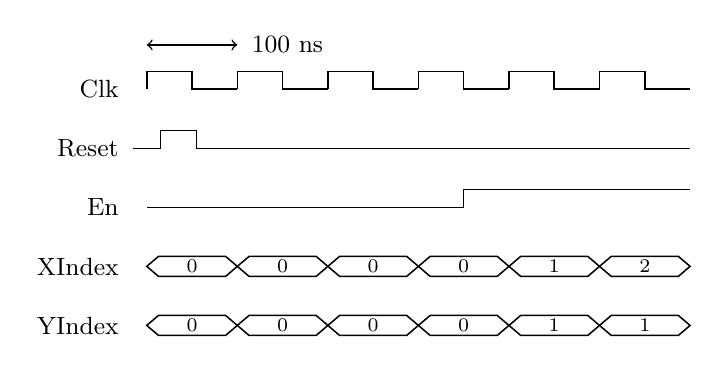
\begin{tikzpicture}[x=1.15cm,y=.75cm,line width=.55pt]
\clockrow{4}{5}
\draw[<->] (0,4.75)--(1,4.75);
\node[font=\small,anchor=west] at (1.05,4.75) {100 ns};
\node[anchor=east,font=\small] at (-.2,3) {Reset};
\draw (-.15,3)--(.15,3)--(.15,3.3)--(.55,3.3)--(.55,3)--(6,3);
\node[anchor=east,font=\small] at (-.2,2) {En};
\draw (0,2)--(3.5,2)--(3.5,2.3)--(6,2.3);
\node[anchor=east,font=\small] at (-.2,1) {XIndex};
\foreach \i/\v in {0/0,1/0,2/0,3/0,4/1,5/2} {\bus{1}{\i}{\v}}
\node[anchor=east,font=\small] at (-.2,0) {YIndex};
\foreach \i/\v in {0/0,1/0,2/0,3/0,4/1,5/1} {\bus{0}{\i}{\v}}
\end{tikzpicture}
\end{center}
\textbf{Continuation of the source timing figure.} Each ellipsis denotes
omitted clock intervals; no extra state is implied by an ellipsis.
\begin{center}\small
\begin{tabular}{c|cccccccccc}\toprule
XIndex & $\cdots$ & COL & 1 & 2 & $\cdots$ & COL & 1 & $\cdots$ & COL & $\cdots$\\
YIndex & $\cdots$ & 1 & 4 & 4 & $\cdots$ & 4 & 7 & $\cdots$ & 7 & $\cdots$\\\bottomrule
\end{tabular}\\[5pt]
\begin{tabular}{c|cc}\toprule
XIndex & COL & 1\\
YIndex & ROW & 1\\\bottomrule
\end{tabular}
\end{center}

\question{4}{15}
Please write a module called ``RowComparator'' that has two modes to
decide the maximum and its position in each mode among the three input
as shown in the figure. Note that if there is unknown or Hi-Z in the
three inputs, the ``Valid'' signal will be low.
\begin{verbatim}
module RowComparator(MaxValue, MaxPos, Valid,
                     In1, In2, In3, iMode);
    input [7:0] In1,In2, In3; // Only one maximum exist
    input iMode; // iMode=0, compare three inputs;
                 // iMode=1, send out center input
endmodule
\end{verbatim}
\textbf{Mode figure.} Mode 0 shades all three positions; Mode 1 shades
only the center position.
\begin{center}
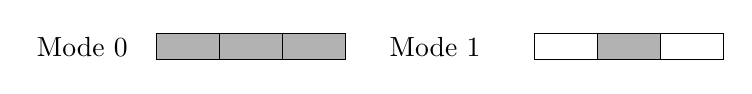
\begin{tikzpicture}[x=.8cm,y=.55cm]
\node[anchor=east] at (-.3,0) {Mode 0};
\foreach \c in {0,1,2} \filldraw[fill=gray!60] (\c,-.3) rectangle (\c+1,.3);
\node[anchor=east] at (5.3,0) {Mode 1};
\foreach \c in {6,7,8} \draw (\c,-.3) rectangle (\c+1,.3);
\filldraw[fill=gray!60] (7,-.3) rectangle (8,.3);
\end{tikzpicture}
\end{center}
\Needspace{16\baselineskip}
\textbf{Input/output example (all original slots, left to right).}
Here x and z are the unknown and high-impedance entries printed in the
figure. Each row below is one column of the original waveform example.
\begin{center}
\begin{tabular}{ccc|c|ccc}\toprule
in1 & in2 & in3 & iMode & Valid & MaxValue & MaxPos\\\midrule
0 & z & 5 & 0 & 0 & 0 & 0\\
0 & 1 & x & 0 & 0 & 0 & 0\\
0 & z & z & 0 & 0 & 0 & 0\\
x & z & 5 & 0 & 0 & 0 & 0\\
1 & 55 & 76 & 0 & 1 & 76 & 3\\
99 & 70 & 51 & 0 & 1 & 99 & 1\\
88 & 89 & 61 & 1 & 1 & 89 & 2\\
9 & 45 & 77 & 1 & 1 & 45 & 2\\
10 & 5 & 3 & 0 & 1 & 10 & 1\\
6 & 22 & 8 & 0 & 1 & 22 & 2\\
93 & 32 & 100 & 0 & 1 & 100 & 3\\\bottomrule
\end{tabular}
\end{center}

\question{5}{20}
Now, we want to process three rows simultaneously that have 9 elements in
total to decide the maximum among the elements in the following three
patterns defined by the shadowed area. Note that you \textbf{must use
``RowComparator''} in Q4. The output signals ``MaxRow'', ``MaxCol''
indicates the position of the maximum and
$1\leq MaxRow,MaxCol\leq3$, where input signal \signal{In2\_3} means the
$2^{\mathrm{nd}}$ column and the third row. If it is the maximum, the
outputs of MaxRow and MaxCol are shown in the figure.
\begin{center}
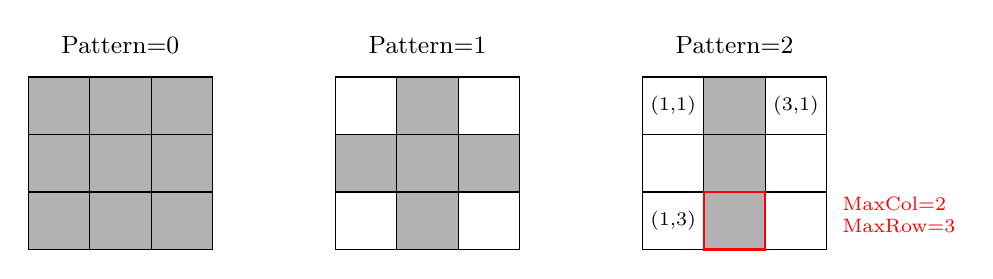
\begin{tikzpicture}[x=.78cm,y=.73cm,font=\small]
\foreach \p/\base in {0/0,1/5,2/10} {
  \node at ({\base+1.5},.55) {Pattern=\p};
  \foreach \r in {0,1,2} \foreach \c in {0,1,2} {
    \pgfmathtruncatemacro{\shade}{(\p==0)||(\p==1 && (\r==1||\c==1))||(\p==2&&\c==1)}
    \ifnum\shade=1\relax
      \fill[gray!60] ({\base+\c},{-\r}) rectangle ({\base+\c+1},{-\r-1});
    \fi
    \draw ({\base+\c},{-\r}) rectangle ({\base+\c+1},{-\r-1});
  }
}
\node[font=\scriptsize] at (10.5,-.5) {(1,1)};
\node[font=\scriptsize] at (12.5,-.5) {(3,1)};
\node[font=\scriptsize] at (10.5,-2.5) {(1,3)};
\draw[red,thick] (11,-2) rectangle (12,-3);
\node[anchor=west,text=red,font=\scriptsize,align=left] at (13.1,-2.4)
  {MaxCol=2\\MaxRow=3};
\end{tikzpicture}
\end{center}
\begin{verbatim}
module PatternComparator3x3(MaxValue, MaxRow, MaxCol, Valid,
    In1_1, In2_1, In3_1, In1_2, In2_2, In3_2,
    In1_3, In2_3, In3_3, Pattern);
    input [7:0] In1_1, In2_1, In3_1;
    input [7:0] In1_2, In2_2, In3_2;
    input [7:0] In1_3, In2_3, In3_3;
    input [1:0] Pattern;

endmodule
\end{verbatim}

\question{6}{13}
Now, we will rely on the inputs generated from the two-dimensional
counter (Count2D) to fetch three consecutive elements from the register
file (RegisterFile) according to the sequence shown in the following
figure. Note that we will put data into the register file through test
bench. You can assume that it contains effective data now. You
\textbf{must use RegisterFile}, to complete the design of module DataFetch.
Note that for clarity, the 2D indexes of TopData, MidData, and BotData are
drawn in the Figure. Actually, the associated values will be sent out.

\Needspace{8\baselineskip}
\textbf{Image-address labels printed in the figure.}
\begin{center}
\begin{tabular}{c|c}\toprule
2D position & Address label\\\midrule
(1,1) & Add=0\\
(COL,1) & Add=COL-1\\
(1,2) & Add=COL\\\bottomrule
\end{tabular}
\end{center}
The image figure also labels its bottom corners (1,ROW) and (COL,ROW).
Its fetch illustration labels Clock=1 at the first column, Clock=2 at
the second column, and Clock=COL+1 at the first column of the next
three-row group. TopData, MidData, and BotData are the three vertical
elements fetched at the same column.

\textbf{Timing figure (redrawn initial portion).} The X entries are the
unknown data intervals in the original. En rises before the first enabled
counter edge, and the first labeled data and Valid occur at the next
edge, marked Clock=1 in the source. A numerical clock period is not
printed in this figure.
\begin{center}
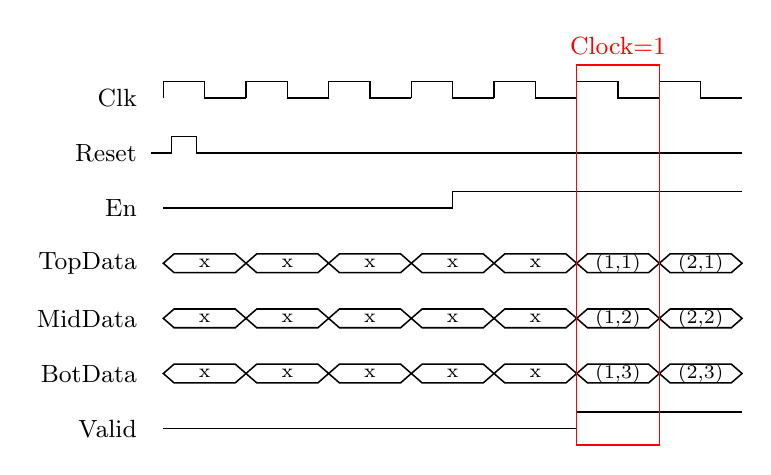
\begin{tikzpicture}[x=1.05cm,y=.7cm,line width=.55pt]
\clockrow{6}{6}
\node[anchor=east,font=\small] at (-.2,5) {Reset};
\draw (-.15,5)--(.1,5)--(.1,5.3)--(.4,5.3)--(.4,5)--(7,5);
\node[anchor=east,font=\small] at (-.2,4) {En};
\draw (0,4)--(3.5,4)--(3.5,4.3)--(7,4.3);
\foreach \row/\label/\ycoord in {3/TopData/1,2/MidData/2,1/BotData/3} {
  \node[anchor=east,font=\small] at (-.2,\row) {\label};
  \foreach \i in {0,...,4} {\bus{\row}{\i}{x}}
  \bus{\row}{5}{(1,\ycoord)}\bus{\row}{6}{(2,\ycoord)}
}
\node[anchor=east,font=\small] at (-.2,0) {Valid};
\draw (0,0)--(5,0)--(5,.3)--(7,.3);
\draw[red] (5,-.3) rectangle (6,6.6);
\node[red,font=\small] at (5.5,6.95) {Clock=1};
\end{tikzpicture}
\end{center}
\textbf{Continuation of the source sequence.}
\begin{center}
\begin{tabular}{c|cccc}\toprule
 & Clock=1 & Clock=2 & $\cdots$ & Clock=COL+1\\\midrule
TopData & (1,1) & (2,1) & $\cdots$ & (1,4)\\
MidData & (1,2) & (2,2) & $\cdots$ & (1,5)\\
BotData & (1,3) & (2,3) & $\cdots$ & (1,6)\\\bottomrule
\end{tabular}
\end{center}
\begin{verbatim}
module DataFetch(Valid, TopData,MidData, BotData,
                 Xindex, YIndex, Clk, Reset);
    input Clk, Reset, En;

    RegisterFile U6_1();

endmodule
\end{verbatim}

\question{7}{20}
Now, please complete the design for maximum search among an 2D image for
a given pattern. (a) Three shift-registers are used each having length of
3 to store the $3\times3$ data of 2D image fetched from register file.
(b) A maximum and its associated X Index (MaxXPos) and Y Index (MaxYPos)
in the 2D image will be generated according to the pattern defined in the
input. Note that the module (\textbf{DataFetch}) \textbf{must be used}.
Note that the ``MaxValid'' will be asserted only when the complete data
in three consecutive rows are all in the shift register for the maximum
search.
\begin{verbatim}
module MaxSearch2D(MaxValue, MaxXPos, MaxYPos, MaxValid,
                  Clk, Reset, En, Pattern);

end
\end{verbatim}
\textbf{System block figure (editable table).}
\begin{center}
\begin{tabular}{ll}\toprule
Block & MaxSearch2D\\
Inputs & Clk, Reset, En, Pattern\\
Internal blocks shown & Count2D, DataFetch\\
Outputs & MaxValue, MaxXPos, MaxYPos, MaxValid\\\bottomrule
\end{tabular}
\end{center}
\textbf{Image example (editable table).} The first highlighted window
spans columns 1--3 and rows 1--3. The next highlighted window spans
columns 2--4 and the same three rows.
\begin{center}
\begin{tabular}{c|rrrr}\toprule
 & $x=1$ & $x=2$ & $x=3$ & $x=4$\\\midrule
$y=1$ & 55 & 168 & 16 & 88\\
$y=2$ & 39 & 39 & 2 & 91\\
$y=3$ & 111 & 15 & 201 & 211\\\bottomrule
\end{tabular}
\end{center}
\textbf{Timing figure (redrawn).} Empty bus cells reproduce empty cells
in the original; no numerical value is assigned to them. The first
highlighted result is 168 at (2,1) with Pattern=2. The next result is
211 at (4,3) with Pattern=0. MaxValid first becomes high at the first
highlighted result. A numerical clock period is not printed in this
figure.
\begin{center}
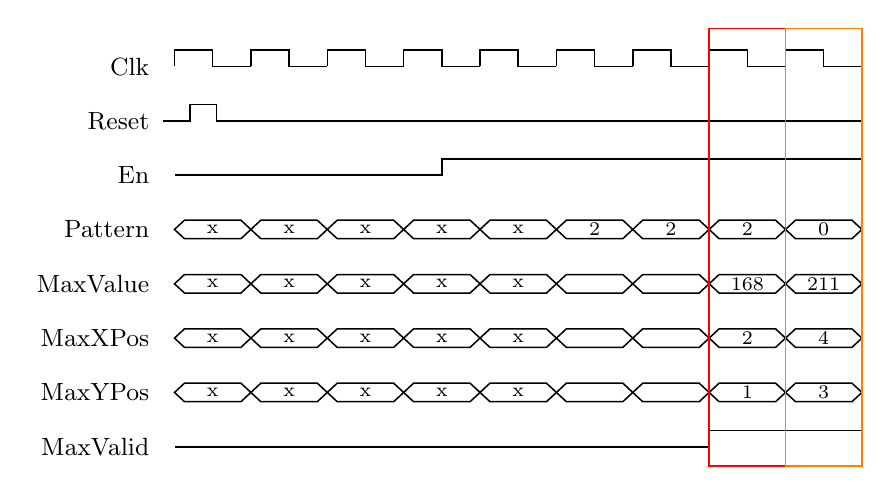
\begin{tikzpicture}[x=.97cm,y=.69cm,line width=.55pt]
\clockrow{7}{8}
\node[anchor=east,font=\small] at (-.2,6) {Reset};
\draw (-.15,6)--(.2,6)--(.2,6.3)--(.55,6.3)--(.55,6)--(9,6);
\node[anchor=east,font=\small] at (-.2,5) {En};
\draw (0,5)--(3.5,5)--(3.5,5.3)--(9,5.3);
\node[anchor=east,font=\small] at (-.2,4) {Pattern};
\foreach \i/\v in {0/x,1/x,2/x,3/x,4/x,5/2,6/2,7/2,8/0} {\bus{4}{\i}{\v}}
\foreach \row/\label in {3/MaxValue,2/MaxXPos,1/MaxYPos} {
  \node[anchor=east,font=\small] at (-.2,\row) {\label};
  \foreach \i in {0,...,4} {\bus{\row}{\i}{x}}
  \bus{\row}{5}{}\bus{\row}{6}{}
}
\bus{3}{7}{168}\bus{3}{8}{211}
\bus{2}{7}{2}\bus{2}{8}{4}
\bus{1}{7}{1}\bus{1}{8}{3}
\node[anchor=east,font=\small] at (-.2,0) {MaxValid};
\draw (0,0)--(7,0)--(7,.3)--(9,.3);
\draw[red] (7,-.35) rectangle (8,7.7);
\draw[orange] (8,-.35) rectangle (9,7.7);
\end{tikzpicture}
\end{center}
\textbf{Shift-register figure (redrawn).} Each shift register has length
3; the input bus is labeled n bits in the source.
\begin{center}
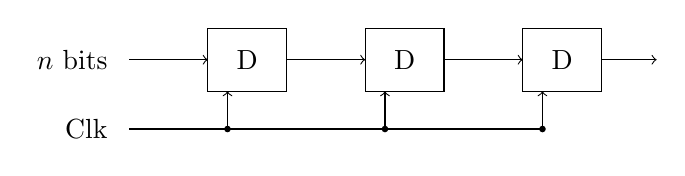
\begin{tikzpicture}[x=1cm,y=.8cm]
\node[anchor=east] at (-.15,.5) {$n$ bits};
\draw[->] (0,.5)--(1,.5);
\foreach \i in {1,3,5} {\draw (\i,0) rectangle (\i+1,1);\node at (\i+.5,.5) {D};}
\draw[->] (2,.5)--(3,.5);\draw[->] (4,.5)--(5,.5);\draw[->] (6,.5)--(6.7,.5);
\draw (0,-.6)--(5.25,-.6);
\node[anchor=east] at (-.15,-.6) {Clk};
\foreach \i in {1,3,5} {
  \draw[->] (\i+.25,-.6)--(\i+.25,0);
  \fill (\i+.25,-.6) circle (1.2pt);
}
\end{tikzpicture}
\end{center}

\Needspace{15\baselineskip}
\bigskip\hrule\smallskip
\textbf{Transcription and provenance note.} This editable LaTeX
transcription was checked against all four pages of
\signal{Final-Exam-2023.pdf}, supplied with this task. The original
\signal{DSD.v} mentioned by the exam was not supplied independently in
this task, so its contents and intended corrections are not claimed to
have been verified. The exam instructions above are historical source
content. Figures are reconstructed using editable tables and TikZ.
Printed wording and interface discrepancies are retained: ``2-dimensiona''
in the introduction; \signal{Rotaor} in Q1; Q6's header omits En even
though the next line declares \signal{input Clk, Reset, En}; Q7 ends
with \signal{end} rather than \signal{endmodule}. Whitespace, line
wrapping, and comment wrapping have been normalized. No unprinted port
widths, memory collision behavior, tie-breaking rules, unknown-mode
behavior, image-boundary rules, or pipeline implementation choices are
added to the source questions. The reproduced snippets are incomplete
exam templates, not compilable Verilog solutions.
\end{document}
